\ifx\wholebook\relax \else
% ------------------------ 

\documentclass{article}
%------------------- Other types of document example ------------------------
%
%\documentclass[twocolumn]{IEEEtran-new}
%\documentclass[12pt,twoside,draft]{IEEEtran}
%\documentstyle[9pt,twocolumn,technote,twoside]{IEEEtran}
%
%-----------------------------------------------------------------------------
%%
% loading packages
%
\newif\ifpdf
\ifx\pdfoutput\undefined % We're not running pdftex
  \pdffalse
\else
  \pdftrue
\fi
%
%
\ifpdf
  \RequirePackage[pdftex,%
            CJKbookmarks,%
       bookmarksnumbered,%
              colorlinks,%
          linkcolor=blue,%
              hyperindex,%
        plainpages=false,%
       pdfstartview=FitH]{hyperref}
\else
  \RequirePackage[dvipdfm,%
             CJKbookmarks,%
        bookmarksnumbered,%
               colorlinks,%
           linkcolor=blue,%
               hyperindex,%
         plainpages=false,%
        pdfstartview=FitH]{hyperref}
  \AtBeginDvi{\special{pdf:tounicode GBK-EUC-UCS2}} % GBK -> Unicode
\fi
\usepackage{hyperref}

% other packages
%-----------------------------------------------------------------------------
\usepackage{graphicx, color}
\usepackage{CJK}
%
% for programming 
%
\usepackage{verbatim}
\usepackage{listings}


\lstdefinelanguage{Smalltalk}{
  morekeywords={self,super,true,false,nil,thisContext}, % This is overkill
  morestring=[d]',
  morecomment=[s]{"}{"},
  alsoletter={\#:},
  escapechar={!},
  literate=
    {BANG}{!}1
    {UNDERSCORE}{\_}1
    {\\st}{Smalltalk}9 % convenience -- in case \st occurs in code
    % {'}{{\textquotesingle}}1 % replaced by upquote=true in \lstset
    {_}{{$\leftarrow$}}1
    {>>>}{{\sep}}1
    {^}{{$\uparrow$}}1
    {~}{{$\sim$}}1
    {-}{{\sf -\hspace{-0.13em}-}}1  % the goal is to make - the same width as +
    %{+}{\raisebox{0.08ex}{+}}1		% and to raise + off the baseline to match -
    {-->}{{\quad$\longrightarrow$\quad}}3
	, % Don't forget the comma at the end!
  tabsize=2
}[keywords,comments,strings]

\lstloadlanguages{C++, Lisp, Smalltalk}

% ======================================================================

\def\BibTeX{{\rm B\kern-.05em{\sc i\kern-.025em b}\kern-.08em
    T\kern-.1667em\lower.7ex\hbox{E}\kern-.125emX}}

\newtheorem{theorem}{Theorem}

%
% mathematics
%
\newcommand{\be}{\begin{equation}}
\newcommand{\ee}{\end{equation}}
\newcommand{\bmat}[1]{\left( \begin{array}{#1} }
\newcommand{\emat}{\end{array} \right) }
\newcommand{\VEC}[1]{\mbox{\boldmath $#1$}}

% numbered equation array
\newcommand{\bea}{\begin{eqnarray}}
\newcommand{\eea}{\end{eqnarray}}

% equation array not numbered
\newcommand{\bean}{\begin{eqnarray*}}
\newcommand{\eean}{\end{eqnarray*}}

\RequirePackage{CJK,CJKnumb,CJKulem,CJKpunct}
% we use CJK as default environment
\AtBeginDocument{\begin{CJK*}{GBK}{song}\CJKtilde\CJKindent\CJKcaption{GB}}
\AtEndDocument{\clearpage\end{CJK*}}

%
% loading packages
%
\newif\ifpdf
\ifx\pdfoutput\undefined % We're not running pdftex
  \pdffalse
\else
  \pdftrue
\fi
%
%
\ifpdf
  \RequirePackage[pdftex,%
       bookmarksnumbered,%
              colorlinks,%
          linkcolor=blue,%
              hyperindex,%
        plainpages=false,%
       pdfstartview=FitH]{hyperref}
\else
  \RequirePackage[dvipdfm,%
        bookmarksnumbered,%
               colorlinks,%
           linkcolor=blue,%
               hyperindex,%
         plainpages=false,%
        pdfstartview=FitH]{hyperref}
\fi
\usepackage{hyperref}

% other packages
%-----------------------------------------------------------------------------
\usepackage{graphicx, color}
%
% for programming 
%
\usepackage{verbatim}
\usepackage{listings}
\usepackage{algorithmic} %for pseudocode
\usepackage{algorithm}


\lstdefinelanguage{Smalltalk}{
  morekeywords={self,super,true,false,nil,thisContext}, % This is overkill
  morestring=[d]',
  morecomment=[s]{"}{"},
  alsoletter={\#:},
  escapechar={!},
  literate=
    {BANG}{!}1
    {UNDERSCORE}{\_}1
    {\\st}{Smalltalk}9 % convenience -- in case \st occurs in code
    % {'}{{\textquotesingle}}1 % replaced by upquote=true in \lstset
    {_}{{$\leftarrow$}}1
    {>>>}{{\sep}}1
    {^}{{$\uparrow$}}1
    {~}{{$\sim$}}1
    {-}{{\sf -\hspace{-0.13em}-}}1  % the goal is to make - the same width as +
    %{+}{\raisebox{0.08ex}{+}}1		% and to raise + off the baseline to match -
    {-->}{{\quad$\longrightarrow$\quad}}3
	, % Don't forget the comma at the end!
  tabsize=2
}[keywords,comments,strings]

\lstloadlanguages{C++, Lisp, Haskell, Python, Smalltalk}

% ======================================================================

\def\BibTeX{{\rm B\kern-.05em{\sc i\kern-.025em b}\kern-.08em
    T\kern-.1667em\lower.7ex\hbox{E}\kern-.125emX}}

\newtheorem{theorem}{Theorem}

%
% mathematics
%
\newcommand{\be}{\begin{equation}}
\newcommand{\ee}{\end{equation}}
\newcommand{\bmat}[1]{\left( \begin{array}{#1} }
\newcommand{\emat}{\end{array} \right) }
\newcommand{\VEC}[1]{\mbox{\boldmath $#1$}}

% numbered equation array
\newcommand{\bea}{\begin{eqnarray}}
\newcommand{\eea}{\end{eqnarray}}

% equation array not numbered
\newcommand{\bean}{\begin{eqnarray*}}
\newcommand{\eean}{\end{eqnarray*}}




\setcounter{page}{1}

\begin{document}

\fi
%--------------------------

% ================================================================
%                 COVER PAGE
% ================================================================

\title{Comparison of imperative and functional implementation of red black tree}

\author{Liu~Xinyu
\thanks{{\bfseries Liu Xinyu } \newline
  Email: liuxinyu95@gmail.com \newline}
%  Tel:   +86-1305-196-8666 \newline}
  }

\markboth{Red black tree}
{imperative and functional implementation}

\maketitle

\ifx\wholebook\relax
\chapter{Comparision of imperative and functional implementation of red black tree}

\section{abstract}
\else
\begin{abstract}
\fi
This post provides the functional and imperative implementation of red black tree. There are
multiple programming languages used, including, C++(on going), Haskell, python and scheme/lisp(on going).
C++ and python are mostly used to show the imperative implementation, while Haskell and Scheme are
used for functional purpose.

It's hard to say if imperative is better than functional and vice versa. Chris Okasaki gave a very expressive implementation for insertion\cite{okasaki}. While the imperative one has better performance.

There may be mistakes in the post, please feel free to point out.

This post is generated by \LaTeXe, and provided with GNU FDL(GNU Free Documentation License).
Please refer to http://www.gnu.org/copyleft/fdl.html for detail.

\ifx\wholebook\relax\else
\end{abstract}
\fi

\vspace{3cm}
{\bfseries Keywords:} Red Black tree, imperative, functional, C++, Haskell, Python, Scheme/Lisp

%{\bfseries Corresponding Author:} Liu Xinyu

\maketitle

% ================================================================
%                 Introduction
% ================================================================
\section{Introduction}
\label{introduction}

Red black tree is one type of the balanced binary search trees. Binary search tree as described
in my previous post\cite{bst-lxy} suffers from below case.

If you try to insert a sequence of number 1, 2, 3, ..., n to a binary search tree. you will get a tree like this.

\begin{figure}[htbp]
       \begin{center}
	\includegraphics[scale=0.5]{img/unbalanced.ps}
        \caption{unbalanced tree} \label{fig:unbalanced-tree}
       \end{center}
\end{figure}

This is a extreme unbalanced binary search tree. In average case, we benifit from binary search tree by $O(log n)$ search time. But in this extream case, the search time is only $O(n)$. It's no better than a normal link-list.

In order to avoid such case, we can shuffle the input sequence by randomized algorithm, such as described in Section 12.4 in CLRS\cite{CLRS}. However, this is not always work, for example the input is fed from user interactively, and the tree need to be built after each input.

Red black tree is one of the most popular and widely used approach to sovle this unbalancing problem. It's a type of self-balancing binary search tree\cite{wiki}. Red black tree is one of the equivalent form of 2-3-4 tree. That is to say, for any 2-3-4 tree, there are at least one red black tree has the same data order. By using color changing and rotation, red black tree provides a very simple and straightforward way to keep the tree balancing.

We call a binary search tree red black tree if it satisfies the following 5 properites\cite{CLRS}.

\begin{enumerate}
\item Every node is either red or black.
\item The root is black.
\item Every leaf (NIL) is black.
\item If a node is red, then both its children are black.
\item For each node, all paths from the node to descendant leaves contain the same number of black nodes.
\end{enumerate}

Why this 5 properties can ensure the red black tree is well balanced? Because they have a key charicteristic, the longest path from root to a leaf can't be as 2 times longer than the shortest path.

Please note the 4th property, which means there won't be 2 adjacent red nodes. so the shortest path only contains black nodes, any paths longer than the shortest one has interval red nodes. According to property 5, all paths have the same number of black nodes, this finally ensure there won't be any path is 2 times longer than others\cite{wiki}.

All read only operations such as search, min/max are as same as in binary search tree. While only the insertion and deletion are special.

This article provides implementation of insertion and deletion for red black tree in C++(on going), Haskell, Python, and Scheme/Lisp(on going) languages. Most imperative algorithms confirms to CLRS\cite{CLRS}. While for functional implementation, thanks for Chris Okasaki very much. He found a very expressive way\cite{okasaki} of insertion.

All completed source code can be downloaded in appendix \ref{appendix}, please refer to appendix for detailed information about build and run.

% ================================================================
% Definition
% ================================================================
\section{Definition}
\label{definition}

The definition of red black tree is very similar to the binary search tree.
In imperative implementation, it has one more color member to denote if the node is red or black. The parent member is critical in red black tree, because
it need back-track in insertion and deletion to keep the balancing properties.
I added some member functions to the definition to help simplify the operations
in node connection change.

\subsubsection*{Python definition, imperative}
\lstset{language=python}
\begin{lstlisting}
RED = 0
BLACK = 1

class Node:
    def __init__(self, key, color = RED):
        self.key = key;
        self.color = color;
        self.left = self.right = self.parent = None

    def set_left(self, x):
        self.left = x
        if x != None:
            x.parent = self

    def set_right(self, x):
        self.right = x
        if x != None:
            x.parent = self

    def set_children(self, x, y):
        self.set_left(x)
        self.set_right(y)

    #parent<->self ==> parent<->y
    def replace_by(self, y):    
        if self.parent is None:
            if y!= None: y.parent = None
        elif self.parent.left == self:
            self.parent.set_left(y)
        else:
            self.parent.set_right(y)
        self.parent = None

    def sibling(self):
        if self.parent.left == self:
            return self.parent.right
        else:
            return self.parent.left

    def uncle(self):
        return self.parent.sibling()

    def grandparent(self):
        return self.parent.parent
\end{lstlisting}

Note that, in case we set a node y as a child of node y, we don't only
make the left or right child point to y, but also make y's parent point to x.
So this is bi-directional assignment. The same thing happens in replace\_by()
member function, when we try to replace a node x with another node y, we
mean make y connect to x's parent as a child. I also provide sibling, uncle,
and grandparent members, those meanings are straightforward.

\subsubsection*{Haskell definition, recursive}
Instead of provide 2 different constructors for red and black node, a color
data is passed to node contructor. It makes the definition very similar to the 
one in binary search tree.

\lstset{language=haskell}
\begin{lstlisting}
data Color = R | B deriving (Show, Eq) 
data RBTree a = Empty
              | Node Color (RBTree a) a (RBTree a)
\end{lstlisting}

% ================================================================
% Rotation and helper functions
% ================================================================
\subsection{Rotation and helper functions} \label{helper-fun}

Rotation is one of the key operations to in red black tree. we know that
different binary search tree can have the data in same order by in-order walk.
Rotation can keep the data order while changing the tree. 

In functional implementation, we can use pattern matching and data construction.
So there is no need to provide rotation functions at all (see below sections).
While the imperative rotation can be simplified a lot by using the member functions we defined.

\subsubsection*{Python rotation functions}
\lstset{language=Python}
\begin{lstlisting}
# (a x (b y c)) ==> ((a x b) y c)
def left_rotate(t, x):
    (parent, y) = (x.parent, x.right)
    (a, b, c)   = (x.left, y.left, y.right)
    x.replace_by(y)
    x.set_children(a, b)
    y.set_children(x, c)
    if parent is None:
        t=y
    return t

# (a x (b y c)) <== ((a x b) y c)
def right_rotate(t, y):
    (parent, x) = (y.parent, y.left)
    (a, b, c)   = (x.left, x.right, y.right)
    y.replace_by(x)
    y.set_children(b, c)
    x.set_children(a, y)
    if parent is None:
        t = x
    return t
\end{lstlisting}

I also provide a function for batch color setting. It accept two lists,
one is list of nodes, the other is list of colors. It helps to set color
to each node in order.

\subsubsection*{Python helper function}
\lstset{language=Python}
\begin{lstlisting}
def set_color(nodes, colors):
    for (n, c) in zip(nodes, colors):
        n.color = c
\end{lstlisting}

% ================================================================
%                 Insertion
% ================================================================
\section{Insertion}

Insertion can violate the red black tree properties, so we need transform
the tree after insertion.

We can use the same insert function as defined in binary search tree, and 
then do some fix the resume the red black properties. One good practice is 
to always insert red node. as far as the new inserted node isn't the root.
We can keep all properties except number 4. It may bring two adjacent red
nodes.

Functional and imperative implementation have different fixing ways. One
is uniformed but has some overhead, the other is a bit complex but has 
higher performance.

\subsubsection*{Haskell red black insertion, functional}
As described by Chris Okasaki, there are total 4 cases which violate property 4.
All of them has 2 adjacent red nodes. However, they have a uniformed form
after fixing\cite{okasaki}. 

\begin{figure}[htbp]
       \begin{center}
	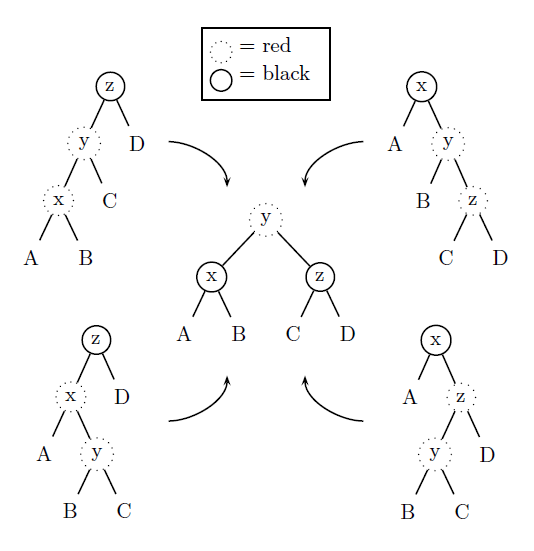
\includegraphics[scale=0.5]{img/insert-fix.eps}
        \caption{4 cases for balancing a red black tree after insertion} \label{fig:insert-fix}
       \end{center}
\end{figure}

Note that this transformation will move the redness one level up. So this is a bottom-up recursive fixing, the last step will make the root node red. According
to property 2, root is always black. So we need final fixing to revert the root
color to black. All these can be implemented as the following Haskell code.

\lstset{language=Haskell}
\begin{lstlisting}
insert::(Ord a)=>RBTree a -> a -> RBTree a
insert t x = makeBlack(ins t x) where  --[1]
    ins Empty x = Node R Empty x Empty --[2]
    ins (Node color l k r) x 
        | x < k     = balance color (ins l x) k r
        | otherwise = balance color l k (ins r x) --[3]
    makeBlack(Node _ l k r) = Node B l k r

balance::Color -> RBTree a -> a -> RBTree a -> RBTree a
balance B (Node R (Node R a x b) y c) z d = 
                Node R (Node B a x b) y (Node B c z d)
balance B (Node R a x (Node R b y c)) z d = 
                Node R (Node B a x b) y (Node B c z d)
balance B a x (Node R b y (Node R c z d)) = 
                Node R (Node B a x b) y (Node B c z d)
balance B a x (Node R (Node R b y c) z d) = 
                Node R (Node B a x b) y (Node B c z d)
balance color l k r = Node color l k r
\end{lstlisting}

Here are some explaination. For [1], the program always set the root
color as black, this is because of property 2; For [2], we always insert
a red leaf to satisify all properties except number 4; For [3], I assume, 
there shouldn't be different nodes with equal key value. But it is not always
applicable. for example in chapter 14, ``Augmenting Data Structures'' in CLRS\cite{CLRS}, it enables such case. The use of otherwise allows user to do this.

In order to test this program, we can write something like below.

\begin{lstlisting}
-- helper function to build a red black tree from a list

listToRBTree::(Ord a)=>[a] -> RBTree a
listToRBTree lst = foldl insert Empty lst

-- Helper function for pretty printing
instance Show a => Show (RBTree a) where
    show Empty = "."
    show (Node c l k r) = "(" ++ show l ++ " " ++ 
                          show k ++ ":" ++ show c ++ " " ++ 
                          show r ++ ")"

main = do
  putStrLn (show (listToRBTree [11, 2, 14, 1, 7, 15, 5, 8, 4]))
  putStrLn (show (listToRBTree [1, 2, 3, 4, 5, 6, 7, 8]))
\end{lstlisting}

This program will output:
\begin{verbatim}
(((. 1:B .) 2:B ((. 4:R .) 5:B .)) 7:B (((. 8:R .) 11:B .) 14:B (. 15:B .)))
(((. 1:B .) 2:B (. 3:B .)) 4:B ((. 5:B .) 6:B (. 7:B (. 8:R .))))
\end{verbatim}

They are trees as shown below.

\begin{figure}[htbp]
       \begin{center}
	\includegraphics[scale=0.5]{img/insert-haskell.ps}
        \caption{Haskell insert results} 
       \end{center}
\end{figure}

\subsubsection*{Python red black tree insertion, imperative}

\lstset{language=Python}
\begin{lstlisting}
def tree_insert(t, key):
    root = t
    x = Node(key)
    parent = None
    while(t):
        parent = t
        if(key < t.key):
            t = t.left
        else:
            t = t.right
    x.parent = parent
    if(parent == None): #tree is empty
        return x
    elif(key < parent.key):
        parent.left = x
    else:
        parent.right = x
    return root
\end{lstlisting}

\subsubsection*{Scheme/Lisp tree insertion, imperative}

\lstset{language=lisp}
\begin{lstlisting}
(define (tree-insert tree x)
  (cond ((null? tree) (list '() x '()))
	((< x (key tree))
	 (make-tree (tree-insert (left tree) x)
		    (key tree)
		    (right tree)))
	((> x (key tree))
	 (make-tree (left tree)
		    (key tree)
		    (tree-insert (right tree) x)))))
\end{lstlisting}

The testing can be refer to section \ref{list2tree}.

\subsection{Deletion}
Deletion is the most complex operation for binary search tree. this is because we
must keep the property, that left sub tree < key < right sub tree. Deleting a node
can break this property very easy.

I don't use the same algorithm described in CLRS\cite{CLRS}, I found a more simple
one from 'Annotated STL'\cite{hj-stl}

The algorithm can be described as below:

To delete a node x from a tree.
\begin{itemize}
\item If x has no child or only one child, splice x out;
\item If x has two children, use minimum of its right to replace x, 
and splice the original minimum out.
\end{itemize}

\subsubsection*{Haskell deletion, recursive}

Haskell version of deletion can be realized by translating the above description
directly into code. But there is a different point, instead of pass a node to the
function, I pass value to be deleted in it. So the program need perform search first.

\lstset{language=Haskell}
\begin{lstlisting}
delete::(Ord a)=> Tree a -> a -> Tree a
delete Empty _ = Empty
delete (Node l k r) x | x < k = (Node (delete l x) k r)
                      | x > k = (Node l k (delete r x))
                      -- x == k
                      | isEmpty l = r
                      | isEmpty r = l
                      | otherwise = (Node l k' (delete r k')) 
                          where k' = key (mint r)
\end{lstlisting}

The test cases and result are shows as below.

\begin{lstlisting}
testDel = "\ntest del 17:\t"++ show (delete t2 17)++
          "\ntest del 7:\t"++ show (delete t2 7)++
          "\ntest del 6:\t" ++ show (delete t2 6)++
          "\ntest del 15:\t"++ show (delete t2 15)++
          "\ntest del non-exist:\t" ++ show (delete t2 5)

main = do
    putStrLn testDel
\end{lstlisting}

\begin{verbatim}
test del 17:    Node (Node (Node (Node Empty 2 Empty) 3 (Node Empty 4 
Empty)) 6 (Node Empty 7 (Node (Node Empty 9 Empty) 13 Empty))) 15 
(Node Empty 18 (Node Empty 20 Empty))
test del 7:     Node (Node (Node (Node Empty 2 Empty) 3 (Node Empty 4 
Empty)) 6 (Node (Node Empty 9 Empty) 13 Empty)) 15 (Node (Node Empty 
17 Empty) 18 (Node Empty 20 Empty))
test del 6:     Node (Node (Node (Node Empty 2 Empty) 3 (Node Empty 4 
Empty)) 7 (Node (Node Empty 9 Empty) 13 Empty)) 15 (Node (Node Empty 
17 Empty) 18 (Node Empty 20 Empty))
test del 15:    Node (Node (Node (Node Empty 2 Empty) 3 (Node Empty 4 
Empty)) 6 (Node Empty 7 (Node (Node Empty 9 Empty) 13 Empty))) 17 
(Node Empty 18 (Node Empty 20 Empty))
test del non-exist:     Node (Node (Node (Node Empty 2 Empty) 3 (Node 
Empty 4 Empty)) 6 (Node Empty 7 (Node (Node Empty 9 Empty) 13 Empty))) 
15 (Node (Node Empty 17 Empty) 18 (Node Empty 20 Empty))
\end{verbatim}

\subsubsection*{C++ deletion, imperative}

C++ version is more complex because it need set the parent properly.
While we can pass the pointer to the node which will be deleted to the function,
so that search is no more needed. The function will return the root
of the result tree.

\lstset{language=C++}
\begin{lstlisting}
template<class T>
node<T>* del(node<T>* tree, node<T>* x){
  if(!x)
    return tree;

  node<T>* root(tree);
  node<T>* old_x(x);
  node<T>* parent(x->parent);

  if(x->left == 0)
    x = x->right;
  else if(x->right == 0)
    x = x->left;
  else{
    node<T>* y=min(x->right);
    x->value = y->value;
    if(y->parent != x)
      y->parent->left = y->right;
    else
      x->right = y->right;

    remove_node(y);
    return root;
  }

  if(x)
    x->parent = parent;

  if(!parent)
    root = x; //remove node of a tree
  else
    if(parent->left == old_x)
      parent->left = x;
    else
      parent->right = x;

  remove_node(old_x);
  return root;
}
\end{lstlisting}

If the node to be deleted is empty, the function simply returns the original tree.
In other cases, it will first record the root of the tree, create a copy pointer
to x, and to its parent.

If either of the children is empty, the program just splice x out. If it has two
none-empty children, we first located the minimum of right child, replace the key
of x to y's, then splice y out. Note that the helper function remove\_node() is
used.

Finally we reset the parent. If the parent pointer we copied before is empty, it
means that we are deleting the root node, so we need return the new root. After
the parent is set properly, we finally remove the old x from memory.

The test cases and result are shows as below.

\begin{lstlisting}
void test_del_n(int n){
  node<int>* empty(0);
  node<int>* t1=clone_tree(tree);
  t1=del(t1, search(t1, n));
  std::cout<<"del "<<n<<":\n"<<tree_to_str(t1)<<"\n";
  assert_("search after del: ", search(t1, n), empty);
  delete t1;
}

test_del_n(17);
test_del_n(7);
test_del_n(6);
test_del_n(15);
test_del_n(1); //try to del a non-exist val
\end{lstlisting}

Because the deletion function in C++ inplace change the tree, so I cloned the test 
tree for each testing. The clone\_tree() function is defined in section \ref{helper-fun}.

The result of these test case is as below.
\begin{verbatim}
del 17:
((((empty), 2, (empty)), 3, ((empty), 4, (empty))), 6, ((empty), 7, 
(((empty), 9, (empty)), 13, (empty)))), 15, ((empty), 18, ((empty), 
20, (empty)))
search after del: 0 OK.
del 7:
((((empty), 2, (empty)), 3, ((empty), 4, (empty))), 6, (((empty), 9, 
(empty)), 13, (empty))), 15, (((empty), 17, (empty)), 18, ((empty), 
20, (empty)))
search after del: 0 OK.
del 6:
((((empty), 2, (empty)), 3, ((empty), 4, (empty))), 7, (((empty), 9, 
(empty)), 13, (empty))), 15, (((empty), 17, (empty)), 18, ((empty), 
20, (empty)))
search after del: 0 OK.
del 15:
((((empty), 2, (empty)), 3, ((empty), 4, (empty))), 6, ((empty), 7, 
(((empty), 9, (empty)), 13, (empty)))), 17, ((empty), 18, ((empty), 
20, (empty)))
search after del: 0 OK.
del 1:
((((empty), 2, (empty)), 3, ((empty), 4, (empty))), 6, ((empty), 7, 
(((empty), 9, (empty)), 13, (empty)))), 15, (((empty), 17, (empty)), 
18, ((empty), 20, (empty)))
search after del: 0 OK.
\end{verbatim}

\subsubsection*{Python deletion, imperative}
Python version is very similar to C++, but it needn't free memory because
of GC support.

\lstset{language=Python}
\begin{lstlisting}
def tree_delete(t, x):
    if (x is None): return t
    [root, old_x, parent] = [t, x, x.parent]
    if (x.left is None):
        x = x.right
    elif (x.right is None):
        x = x.left
    else:
        y = tree_min(x.right)
        x.key = y.key
        if (y.parent != x):
            y.parent.left = y.right
        else:
            x.right = y.right
        remove_node(y)
        return root
    if (x != None):
        x.parent = parent
    if (parent != None):
        root = x
    else:
        if(parent.left == old_x): parent.left = x
        else: parent.right = x
    remove_node(old_x)
    return root
\end{lstlisting}

This function can be tested as below:

\begin{lstlisting}
def __test_del_n(self, n):
    t = clone_tree(self.tree)
    t = tree_delete(t, tree_search(t, n))
    print "del ", n, ": ", tree_to_str(t)
    self.__assert("search after del: ", tree_search(t, n), None)

def test_del(self):
    self.__test_del_n(17)
    self.__test_del_n(7)
    self.__test_del_n(6)
    self.__test_del_n(15)
    self.__test_del_n(1) #del a non-exist value
\end{lstlisting}

The test result is as same as C++.

\subsubsection*{Scheme/Lisp deletion, recursive}

\lstset{language=lisp}
\begin{lstlisting}
(define (tree-delete tree v)
  (cond ((null? tree) tree)
	((< v (key tree)) (make-tree (tree-delete (left tree) v)
				     (key tree)
				     (right tree)))
	((> v (key tree)) (make-tree (left tree)
				     (key tree)
				     (tree-delete (right tree) v)))
	((null? (left tree)) (right tree))
	((null? (right tree)) (left tree))
	(else (let ((newkey (key (tree-min (right tree)))))
		(make-tree (left tree)
			   newkey
			   (tree-delete (right tree) newkey))))))
\end{lstlisting}

Test cases are like the following.

\begin{lstlisting}
(define (test-del)
  (display (tree-delete t1 17)) (newline)
  (display (tree-delete t1 7)) (newline)
  (display (tree-delete t1 6)) (newline)
  (display (tree-delete t1 15)) (newline)
  (display (tree-delete t1 5)))
\end{lstlisting}

It will output the result in emulator as below.

\begin{verbatim}
(test-del)
((((() 2 ()) 3 (() 4 ())) 6 (() 7 ((() 9 ()) 13 ()))) 15 (() 18 (() 20 ())))
((((() 2 ()) 3 (() 4 ())) 6 ((() 9 ()) 13 ())) 15 ((() 17 ()) 18 (() 20 ())))
((((() 2 ()) 3 (() 4 ())) 7 ((() 9 ()) 13 ())) 15 ((() 17 ()) 18 (() 20 ())))
((((() 2 ()) 3 (() 4 ())) 6 (() 7 ((() 9 ()) 13 ()))) 17 (() 18 (() 20 ())))
((((() 2 ()) 3 (() 4 ())) 6 (() 7 ((() 9 ()) 13 ()))) 15 ((() 17 ()) 18 (() 
20 ())))
;Unspecified return value
\end{verbatim}

\section{Randomly built binary search tree}
In CRLS\cite{CLRS}, it described about randomly built binary search tree.
Ramdomly building can help to avoid (decrease the possibility) unbalanced
binary trees.

This can be easily implemented in imperative way, such as by C++ and Python.
Before call build\_tree() or list\_to\_tree() function, we can call random
process, to shuffle the list or collection. The same approach can also be
used in Scheme/Lisp. While for pure functional programming language, such as
Haskell, randomization violate the property of pure function. We have to
use alternative approach such as Monad.

There are more solution to ensure the tree is balanced, such as red black tree,
please refer to other posts for detailed implementation.

\section{Appendix} \label{appendix}
%\appendix
All programs are provided along with this article. They are free for downloading.
\begin{itemize}
\item bstree.cpp, C++ version of binary seach tree, including all test cases. I 
compiled and tested it with GUN G++ 3.4.4.
\item BSTree.hs, Haskell version of binary search tree, with test cases. I compiled
and tested it with GHC 6.10.4.
\item bstree.py, Python version of the binary search tree, with test cases. Tested
with Python 2.5.1
\item bstree.scm, Scheme version of the binary search tree and test cases. Tested
with MIT/Scheme 14.9
\end{itemize}
download position: http://sites.google.com/site/algoxy/bstree/bstree.zip

\begin{thebibliography}{99}

\bibitem{CLRS}
Thomas H. Cormen, Charles E. Leiserson, Ronald L. Rivest and Clifford Stein. 
``Introduction to Algorithms, Second Edition''. ISBN:0262032937. The MIT Press. 2001

\bibitem{okasaki}
Chris Okasaki. ``FUNCTIONAL PEARLS Red-Black Trees in a Functional Setting''. J. Functional Programming. 1998

\bibitem{bst-lxy}
Liu Xinyu. ``Comparison of imperative and functional implementation of binary search tree''. http://sites.google.com/site/algoxy/bstree

\bibitem{wiki}
Wikipedia. ``Red-black tree''. http://en.wikipedia.org/wiki/Red-black\_tree

\bibitem{hj-stl}
Hou Jie. ``The annotated STL sources (using SGI STL)''. ISBN:7-5609-2699-1 http://press.hust.edu.cn. 2002.

\bibitem{literal-program}
http://en.literateprograms.org/Category:Binary\_search\_tree

\bibitem{wiki-fold}
http://en.wikipedia.org/wiki/Foldl

\end{thebibliography}

\ifx\wholebook\relax\else
\end{document}
\fi
